\chapter{Microservice - Governance - Observability}

Die Microservicearchitektur wurde erstmals 20XX von XXXX \marginpar{TODO: Quelle finden} vorgeschlagen. Dabei wurden wichtige Elemente aus dem Vorgänger, der \ac{SOA} übernommen. Außerdem stellt diese Architektur einen Nachfolger für den monolithischen Architekturansatz dar. Im folgenden Teil soll anhand eines kurzes Beispiels erläutert werden, welche Aspekte der einzelnen Ansätze in die Microservicearchitektur einspielen.\autocites{Ren2018}{Mazlami2017}{Escobar2016}

\section{Die Geschichte der Microservicearchitektur}

Applikationen dienen als Automatisierer und sollen helfen komplexe Prozesse einfacher und am besten ohne menschliches Zutun beenden zu können. Dabei besitzt die Applikation Aufgaben, die aus der Gesamtheit des Prozesses erwachsen. Es kann also sein, dass Daten aus vielen verschiedenen Bereichen eines Unternehmens benötigt werden. Anhand eines vereinfachten Prozesses sollen nun die verschiedenen Architekturen abgeleitet werden. Im Beispiel wird ein Online-Shop dargestellt.

\begin{figure}[h]
	\centering
	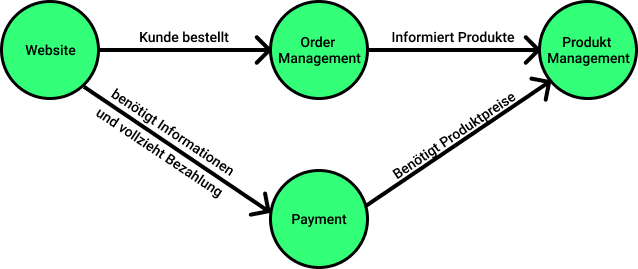
\includegraphics[width=1.0\linewidth]{img/prozess_eCommernce.png}
	\caption[Prozess Online-Shop]{Vereinfachter Prozess eines Online-Shops mit vier Komponenten\\ Quelle: Eigen}
	\label{fig:prozess_online_shop}
\end{figure}

In Abbildung \vref{fig:prozess_online_shop} ist der Prozess beschrieben. Es wird dabei nur ein einfacher Bestellprozess betrachtet. Ein Kunde bestellt auf einer Website bestimmte Produkte. Im Order-Management werden dann die Informationen zu den entsprechenden Produkten, die zu dieser Bestellung gehören aus dem Produkt-Management angefordert. Mithilfe der Produktinformationen kann dann im Bezahlbereich ein Endpreis für den Nutzer kalkuliert werden. Die dort generierten Informationen können dann wieder der Website zur Verfügung gestellt werden, damit der Nutzer einen Bezahlvorgang einleiten kann.

\subsection{Monolithen}
Wird nun ein Entwicklerteam damit beauftragt ein System auf Basis dieses Prozesses zu implementieren so kann ein \textbf{monolithischer Ansatz} gewählt werden. Eine ebenfalls vereinfachte Architektur könnte für den oben beschriebenen Prozess folgendermaßen aussehen\autocites{Chen2017}{de2019monolithic}:

\begin{figure}[h]
	\centering
	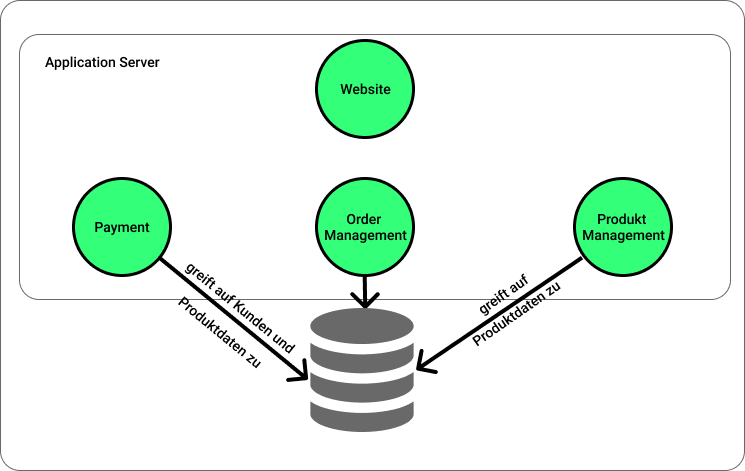
\includegraphics[width=1.0\linewidth]{img/monolitische_architektur.png}
	\caption[monolitische Architektur]{Abbildung des Prozesses mithilfe eines monolithischen Ansatzes\\Quelle: Eigen}
	\label{fig:monolithic_arch}
\end{figure}

Die in \vref{fig:monolithic_arch} beschriebene Architektur hat einige Eigenschaften, die charakteristisch für monolithische Architekturen sind. Dazu gehört unter anderem die Tatsache, dass der Prozess in verschiedene Komponenten oder Module unterteilt wird, welche alle zusammen die Applikation bilden. Zusätzlich greifen alle Komponenten, welche als eine Einheit auf einem Server liegen, auf dieselbe Datenbank zu. Außerdem werden die verschiedenen Bestandteile in Komponenten unterteilt, welche alle im selben Prozess laufen. Dies ermöglicht das einfache Teilen von Objekten, da sich alle Komponenten denselben Speicher teilen. Beides sind Merkmale, die charakteristisch für eine monolitische Applikation sind. Ein Vorteil dieses Ansatzes ist, dass die Kommunikation zwischen den verschiedenen Komponenten sehr einfach ist, da diese meistens auch logisch als \textit{ein Programm} ablaufen. So kann das Order-Management Daten anfordern indem es eine Methode im Produkt-Management aufruft. Ein Nachteil dieses Ansatzes besteht aber darin, dass eine sehr starke Kohäsion und Abhängigkeit von der spezifischen Implementierung einer Komponente besteht. So kann beispielsweise das Order-Management nur ausgestauscht werden, wenn unter viel Aufwand auch alle anderen Komponenten in dem Monolithen angepasst werden. 

\begin{definition}[Monolith]
	Monolithen lassen sich anhand folgender Eigenschaften definieren: \autocite[S. 3]{microservice_enterprise}
	\begin{enumerate}
		\item Monolithen werden als einzelne Einheit entworfen, entwickelt und deployt. Das bedeutet, dass sie oftmals eine enorme Komplexität erreichen, welche schwer nur schwer verwaltet werden kann.
		\item Die einzelnen implementierten Businessfunktionen können nicht einzeln skaliert oder aktualisiert werden. Alle Komponenten sind ein zentrales Deployment des gesamten Monolithen gebunden, auch wenn nur eine Komponente aktualisiert werden muss.
		\item Die initiale Wahl einer Programmiersprache kann später nicht mehr oder nur sehr schwer wieder geändert werden, da jede einzelne Folgeentscheidung auch auf Basis dieser Wahl getroffen wurde.
		\item Bei Instabilität einer einzelnen Komponenten besteht die Gefahr, dass die gesamte Applikation einen Fehler erleidet und nicht mehr funktionsfähig ist.
	\end{enumerate}
\end{definition}

\subsection{SOA und ESB}

Eine Lösung für die Nachteile, die ein Monolith mit sich bringt sollte mithilfe der \ac{SOA} erreicht werden. Die \ac{SOA} versucht, die große, schwer skalierbare und stark zusammenhängende Einheit eines Monolithen aufzubrechen in kleine \enquote{self-contained} Services. Diese Services haben einen klar definierten Aufgabenbereich und besitzen ein wohldefiniertes Interface, welches \textbf{unabhängig} von der unterliegenden Implementierung ist. Dies löst bereits mehrere Probleme, welche in einem Monolithen vorhanden waren. So kann nun durch die lose Kopplung zwischen den Services (Komponenten in dem Monolithen) eine individuellere Skalierbarkeit erreicht werden. Jetzt steht aber nicht mehr nur ein zentraler Endpunkt wie bei dem Monolithen zur Verfügung der von einem Client angesprochen werden kann. Deshalb stellt sich die Frage, wie bestimmt werden kann, welche Instanz eines Services angesprochen werden soll, wenn dieser repliziert vorliegt. Um unter anderem dieses Problem zu lösen, wird die \ac{SOA} meistens nur in Verbindung mit einem \ac{ESB} verwendet.

Unter einem \ac{ESB} kann man sich vereinfacht eine Art intelligenten Load-Balancer vorstellen. Zu den klassischen Aufgaben eines \ac{ESB} gehören unter anderem die Weiterleitung der Anfragen eines Clients zu den richtigen Services. Der Grund warum es sich bei dem \ac{ESB} um einen intelligenten Load-Balancer handelt ist, weil er zusätzlich die Fähigkeit besitzt einzelne Services zu zusammengesetzten logischen Einheiten zu kombinieren. Wie diese Services kombiniert werden obliegt dabei dem Implementierenden, welcher es auf Basis des zu implementierenden Prozesses entscheiden kann. Zusätzlich können in einem \ac{ESB} noch Funktionen wie beispielsweise Authentifizierung von Clients oder auch Monitoringfunktionen eingebaut werden.

Das oben eingeführte Beispiel könnte in einer \ac{SOA} folgendermaßen umgesetzt werden:
\begin{figure}[h]
	\centering
	\caption{TODO: Hier kommt noch das Bild der SOA Arch hin}
\end{figure}

Diese nächste \enquote{Entwicklungsstufe} auf dem Weg zur Microservicearchitektur lässt sich also mithilfe folgender Eigenschaften definieren:

\begin{definition}[SOA und ESB]
	Im Rahmen der \ac{SOA} ist ein Service mit folgenden Eigenschaften definiert: \autocite[S. 4]{microservice_enterprise}
	\begin{enumerate}
		\item Ein Service ist eine eigenständige Implementierung einer wohldefinierten Businessfunktion, welcher über das Netzwerk erreichbar ist. Sie sind lose gekoppelt und verfügen über ein wohldefiniertes Interface über welches sie nach außen hin ansprechbar sind, somit sind sie implementierungsunabhängig. Services stellen die Grundbausteine innerhalb der \ac{SOA} dar.
		\item Zusammengesetzte Services können auf Basis bestehender Services generiert werden und erben alle Eigenschaften, die ein Service auch hat.
		\item Services können dynamisch registriert werden. Es ist oftmals für den Client nicht relevant die genaue Adresse eines Services zu kennen, da diese im Rahmen einer Service-Registry in Form von Metadaten vorliegen.
	\end{enumerate}
	Dem \ac{ESB} fällt dabei die Rollen eines intelligenten Mittelsmann (\enquote{smart Pipeline}) zu. Er besitzt die Möglichkeit Services zusammenzufassen und sich um die Sichtbarkeit, sowie die zusätzliche Bereitstellung von Funktionen zu kümmern. Er stellt einen zentrale Schnittstelle zwischen den einzelnen Services und der \enquote{Außenwelt} innerhalb der \ac{SOA} dar.
\end{definition}

\subsection{Der letzte Schritt - die Microservicearchitektur}
\autocite{Silveira2016}
% TODO: Microservices noch endgültig definieren



%%%%%%%%%%%%%%%%%%%%%%%
%	OBSERVABILITY	  %
%%%%%%%%%%%%%%%%%%%%%%%
\section{Observability}

Der Begriff und der Nutzen von Observability für Services lässt sich anhand der folgenden Zitate sehr gut nachvollziehen:

\begin{quote}
	\enquote{Collecting data is cheap, but not having it when you need it can be expensive.}\autocite[S. 373]{microservice_enterprise} - \textit{\citeauthor{microservice_enterprise}}

	\enquote{Observability is the measure of how well internal states [...] of a system can be inferred by knowledge of its external outputs [...].}\autocite[S. 35]{Yordanova2016} - \textit{\citeauthor{Yordanova2016}}
\end{quote}

Innerhalb einer jeden Technologie wird uns durch Standards \marginpar{CNCF} ermöglicht wichtige Einsichten in Services zu erhalten. Wird jedoch darauf verzichtet Daten aus einem Service zu sammeln, so kann es im Fehlerfall die Konsquenz haben, dass Fehler erst garnicht entdeckt oder bemerkt, geschweige denn gelöst werden. Es ist also von essenzieller Bedeutung Services zu observieren. Nun kommt die Frage auf, was genau ist Observability? Welche Aspekte meines Services müssen überwacht werden, um einen Fehlerfall schnell bemerken zu können und diesen dann durch die gesammelten Daten analysieren zu können?\\
In \citetitle{Sridharan2018} wird beschrieben, wie sich Services in verteilten Systemen observieren lassen. Dazu nimmt der Autor eine Unterteilung in drei Säulen vor.

\begin{definition}[Die drei Säulen der Observability]\autocites[Chapter 4: Three Pillars of Observability]{Sridharan2018}[S. 373f]{microservice_enterprise}
	Um erfolgreich auf interne Zustände schließen zu können, müssen Daten existieren auf deren Basis Schlussfolgerungen gezogen werden können. Diese Daten werden mithilfe der drei Säulen erhoben und verarbeitet:

	\newcounter{pillarsCounter}

	\begin{enumerate}
		\item \textbf{Logging:}\\
		Das Ziel des Loggings besteht darin, Ereignisse zu dokumentieren. Es ist dabei nicht von Bedeutung, um welche Ereignisse es sich handelt. Zusätzlich zu den eigentlichen Daten des Ereignisses, welche unterschiedlichster Art sein können, ist es möglich Metadaten zu loggen, welche dem Ereignis zusätzlichen Kontext verleihen oder einen sonstigen Mehrwert bieten. Dazu gehören z.B. Information zum Zeitpunkt des Ereignisses (\textit{timestamp}), Ergebnis des Ereignisses (\textit{status}), usw. 
		
		Ein Vorteil des Loggings bestehen unter anderem darin, dass Logs extrem einfach zu generieren sind. Ein Nachteil des Loggings besteht darin, dass Logs an sich keine zusätzliche Aussagekraft haben, außer ihrem direkten Inhalt. Es ist schwer rein anhand von Logs ein komplexes Fehlerbild in einem verteilten System zu finden und korrekte Maßnahmen zur Behebung zu treffen.
		\item \textbf{Metriken:}\\
		Metriken stellen eine numerische Repräsentation von Daten dar, welche über bestimmte Zeitintervalle gemessen wurden. \autocite[S. 373f]{Sridharan2018} Metriken können also als Indikatoren verwendet werden, um herauszufinden, wie ein Service performt. Bekannte Metriken sind z.B. die Anzahl der Anfragen, die ein Service in einer Minute verarbeitet, oder die durchschnittliche Antwortzeit eines Services (seine Latenz). Das zweite Beispiel zeigt sogar ein Zusammenspiel zwischen zwei Säulen auf. Diese Metrik kann als abgeleitete Eigenschaft aus Daten des Loggings interpretiert werden, da die Latenz als Differenz zwischen dem Zeitpunkt der Anfrage und dem Zeitpunkt der Antwort ist.
		\setcounter{pillarsCounter}{\value{enumi}}
	\end{enumerate}

	\textbf{Logging} kann also als datenaggregierende Säule angesehen werden. \textbf{Metriken} hingegen nutzen (unter anderem) die aggregierten Daten, um neue wertvollere Informationen abzuleiten. Die Kombination zwischen diesen beiden Säulen bietet einem Außenstehenden einen guten Einblick in den internen Zusatand \textit{eines} Services. Wie bereits bei der Defintion eines Microservices erwähnt, ist es aber nicht unüblich hunderte kleine Services beobachten zu müssen. Es wäre allerdings sehr unpraktisch nur die einzelnen Services in Isolation zu betrachten, da es sich um stark vernetzte und voneinander abhängige Services handelt. Deshalb existiert noch eine dritte Säule, um auch serviceübergreifend Daten zu aggregieren und diese zu verwertbaren Informationen umzuwandeln.

	\begin{enumerate}
		\setcounter{enumi}{\value{pillarsCounter}}
		\item \textbf{Tracing:}\\
		Betrachtet man die bisherigen Säulen, so lässt sich ein Trend auf der Betrachtungsebene feststellen. Das Logging fokussiert sich auf die Sammlung der Daten einzelner Ereignisse - der kleinsten Einheit. Die Metriken arbeiten nun ereignisübergreifend und wandeln die Daten zu nutzbaren Informationen um, damit Einsichten in das Verhalten eines Services vorhanden ist - die mittlere Einheit. Der nächste logische Schritt wäre nun, da Services in einem verteilten System miteinander vernetzt sind, eine Anfrage von Beginn bis zur endgültigen Antwort serviceübergreifend zu observieren, quasi eine End-to-End Betrachung. Genau diese Betrachtung wird mithilfe von Tracing ermöglicht. Eine \textit{Trace} (\enquote{Spur}) ist eine Liste zusammenhängender, verteilter Ereignisse, welche als Repräsentant einer End-to-End Anfrage angesehen werden können.
	\end{enumerate}

\end{definition}
Mithilfe dieser drei Säulen ist es nun einem Außenstehenden möglich auf \enquote{die inneren Zustände eines Systems auf Basis seiner Ausgaben} zu schließen. Dazu ein kurzes Beispiel:\\
Es wird ein Fehler bei einer Anfrage regisitriert. Der dafür zuständige Mitarbeiter kann nun mithilfe des \textbf{Tracings} feststellen um welchen Request es sich handelt. Dabei erkennt er, welche Services als Ursache für den Fehler infragekommen. Im nächsten Schritt kann er sich einzelne \textbf{Metriken} der Services ansehen, um eventuell eine Anomalie festzustellen. Im letzten Schritt kann er durch Ansehen der \textbf{Logs} eine genaue Fehlerursache feststellen.


\section{Governance}

Nun können Services observiert werden und ein Unternehmen kann sicherstellen, dass Fehler gefunden werden können, wenn sie auftreten. Ein identifizierter Fehler muss danach an das richtige Team weitergeleitet werden, sodass dieser schnellstmöglich behoben werden kann. Der Vorgang des Findens des Veranwtortlichen ist von immenser Bedeutung, da dort auch die Expertise für einen bestimmten Service liegt. Dies stellt einen wichtigen Teilbereich der Governance dar \autocite[S. 6]{bavskarada2018architecting}. Eine klare Defintion der Zuständigkeiten gestaltet sich aber bei größeren Unternehmen und einer hohen Anzahl an Services immer schwieriger. Im folgenden Abschnitt wird versucht grundlegende Bestandteile von Microservice Governance herauszuarbeiten, sodass klar ist, was darunter zu verstehn ist.

In \citetitle{microservice_enterprise} wird beschrieben, dass viele Konzepte, welche für die Governance mit \ac{SOA} entwickelt wurden, auch auf Microservices anwendbar sind. Um zu verstehen, worum es sich bei Governance überhaupt handelt, wird zuerst eine Wortdefinition genutzt:

\begin{definition}[Governance] Dazu wird zunächst eine Defintion aus dem Camebrigde Wörterbuch entnommen:
	\enquote{the way that organizations or countries are managed at the highest level, and the systems for doing this}\autocite{camebdrigeGovernance}
\end{definition}

Bei Governance handelt es sich also um Möglichkeiten, wie Organisationen verwaltet werden. Nun stellt sich die Frage, wie sich Governance in der IT abbilden lässt und was genau es im Bezug auf Microservice Governance bedeutet. Software und insbesondere Microservices müssen verwaltet werden. Vor allem bei der hohen Anzahl an Microservice ist eine klare Form der Verwaltung wichtig. Um Services erfolgreich verwalten zu können sind einige Elemente zentral zu verwalten. Es kann allerdings nicht alles zentral verwaltet werden, wie es bei Monolithen der Fall war. Eine zentrale Verwaltung bietet sich genau dann an, wenn ein fest vorgeschriebenes Toolset in einer (oder wenigen) Programmiersprachen genutzt wird. Bei Microservices steht es dem implementierenden Team frei, die Technologie zu wählen, die ihnen für den Anwendungsfall am passensten erscheint. Dies führt in der Governance allerdings zu Problemen, da es für ein Unternehmen nicht möglich ist, für jede mögliche Kombination von Tools entsprechende Standards festzulegen. Deshalb gibt es die sogenannte \textit{dezentralisierte Governancen}, damit Unternehmen einen Teil zentral verwalten können, und andere wichtige Teile dezentral von den Entwicklerteams entschieden werden können\autocite[Kapitel 2]{di2017research}.

\begin{definition}[Dezentralisierte Governance]
	Dezentrale Governance bedeutet, dass Services in folgenden Punkten nicht zentral gesteuert werden, sondern von den Entwicklerteams übernommen werden:\autocites[S. 154]{microservice_enterprise} [Decentralized Governance]{FowlerMicrservices}
	
	\begin{itemize}
		\item \textbf{Entwurf eines Services:}\\
		Der Entwurf eines Services wird nicht zentral gesteuert. Dies steht ganz im Rahmen der Defintion eines Microservice, da die Entscheidung über die sinnvollsten Technologien für die Aufgabe bei den Entwicklern liegen soll. Es gilt bei dem Design bereits darauf zu achten, welche Schnittstellen und Abhängigkeiten der eigene Service hat, um später schnelle Fortschritte während der Entwicklung machen zu können.
		\item \textbf{Entwicklung eines Services:}\\
		Auch die Entwicklung eines Services muss vom zuständigen Team überwacht werden. Dies ermöglicht schnellere Entscheidungen und einfachere Prozesse. So muss auch bei Problemen nicht ein Umweg über eine höhere Instanz gewählt werden, sondern es kann direkt mit dem zuständigen Team der Abhängigkeit gesprochen werden.
		\item \textbf{Deployment eines Services}:\\
		Befindet sich ein Service nun in der Entwicklung, ist es wichtig schnell einen möglichst automatisierten Ansatz für das Deployment des Services aufzubauen. Auch hier ist es von Vorteil, dass es eine dezentral organisierte Komponente ist, da aufgrund der freien Wahl der Programmiersprache und der Technologie entsprechendes Tooling verwendet werden muss. Auch kommt es immer auf die Art und den Inhalt des Services an, welcher auch Anforderungen an das Deployment stellen kann.
	\end{itemize}
	Im Gegensatz zu diesen Elementen gibt es auch in der dezentralen Governance Elemente, welche zentral verwaltet werden müssen. Dazu zählen \autocite[S. 154]{microservice_enterprise}:

	\begin{enumerate}
		\item die Observability
		\item eine Service-Registry und Service-Discovery
		\item das API-Management und
		\item die Entwicklungszyklen
	\end{enumerate}

	
\end{definition}

Dieses Konzepte der dezentralen Verwaltung von servicespezifischen Aufgaben ermöglicht es den Teams die Idee von Microservices umzusetzen. Sie haben die Chance ohne Einschränkungen seitens des Unternehmens den Technologieverbund zu wählen, welcher ihnen für den Anwendungsfall am sinnvollsten erscheint. Trotz dieser Freiheit entsteht kaum ein Tradeoff dabei, da weiterhin zentrale Komponenten zur Kontrolle und Steuerung exisiteren, welche mit jedem Service kompatibel sind. Dies wird unter anderem durch das Verwenden von offenen Standards ermöglicht, sodass eine große Reihe an Tools miteinander kompatibel sind.

Es lässt sich also feststellen, dass trotz der dezentralen Natur von Microservice einige Komponenten sinnvollerweise zentral angelegt werden\autocite[S. 155ff]{microservice_enterprise}.

\section{Eine Lücke zwischen Governance und Observability}

Im vorherigen Abschnitt wurden einige potenzielle Problempunkte beim Nutzen einer Microservicearchitektur identifiziert. Es sticht vor allem heraus, dass es für einen Verantwortlichen nur sehr schwer möglich ist fundierte Risikoeinschätzungen abzugeben. Es stellt sich im unternehmerischen Alltag oftmals die Frage, wer einen Fehler im System beheben muss. Diese Frage kann genau dann beantwortet werden, wenn klar ist wo der Fehler liegt. Im Abschnitt über Observability sind mithilfe der drei Säulen Möglichkeiten geschaffen einen fehlerhaften Service zu finden. Trotzdem kann auch mithilfe dieser Informationen nicht unbedingt immer die Ursache des Fehlers ausfindig gemacht werden. Ein sehr häufiges Ergebnis bei der Fehleranalyse im Kontext verteilter Systeme ist, dass mehr als ein Service als Fehlerursache in Frage kommt. Das bedeutet, dass der zuständige Mitarbeiter für die Fehleridentifizierung mit mehreren Teams in Kontakt treten muss und diese dann den Fehler in ihren Services so schnell wie möglich beheben können. \\
Auch und vor allem bei Fehlern in einer Software als Kernbestandteil eines Unternehmens greift eine altbekannte Redensart: \textit{Zeit ist Geld}. Dass Zeit wirklich Geld bedeuetet und die Zeit, die bis zum Beheben eines Fehlers vergeht, so kurz wie möglich gehalten werden muss, zeigen Zahlen eines Ausfalls der Amazon Website aus dem Jahr 2016. Dort führte eine Nichterreichbarkeit der Website für nur 20 Minuten zu einem Verlust von ca 3.5 Mio Euro \marginpar{QUELLE}.

An dieser Stelle, einer Schnittstelle zwischen Governance und Observability gilt es so wenig Zeit wie möglich zu verschwenden, um mehr Zeit bei der eigentlichen Fehlerbehebung zur Verfügung zu haben. Es sollte also innerhalb eines Unternehmens eine Möglichkeit geben diese Informationen schnell aufzufinden. Im Folgenden werdene einige Anforderungen herausgestellt, welches ein Tools haben muss, um in diesem Schnittstellenbereich einen positiven Einfluss auf die Fehlerbehebung zu haben.


\section{Anforderungen an das Konzept}\label{chap:Anforderungen}

Ein Tool, das sich in diese Lücke einfügt, benötigt sowohl Komponenten aus dem eher der Governance zuzuschreibenden Bereich, als auch Elemente aus der Observability.

\begin{enumerate}

\item \textbf{\enquote{Zeit ist Geld}:}\\
Im vorherigen Kapitel wurde diese Redensart bereits genutzt, um einen wichtige Anforderung zu verdeutlichen. Die Geschwindigkeit, in der ein Fehler innerhalb von Software identifiziert und behoben werden kann, ist maßgeblich entscheidend für die Auswirkungen und die Tragweite des Fehlers. Die Auswirkungen sind nicht immer nur finanzieller Natur. Auch im Falle von Sicherheitslücken in einem System gilt es den Ursprung eines Angriffs schnellstmöglich identifizieren zu können, um auch hier den Schaden möglichst gering zu halten. Wird also ein Tool entwickelt, dass in einem solchen Fall zur Anwendung kommt, muss es dem Endnutzer eine einfache, schnelle Möglichkeit bieten, die Ursache eines Fehlers unter hunderten möglichen Services zu finden. \\
Das Finden des Services leitet auch direkt zum nächsten elementaren Bestandteil eines solchen Tools über.

\item \textbf{Bereitstellen von Informationen - nicht nur generieren von Daten:}\\
Ein solches Tool hat auch die Aufgabe, generierte Daten, seien es spezielle, extra gesammelte, oder bereits vorhandene durch andere Tools zur Verfügung gestellte Daten so aufzubereiten, dass nutzbare Informationen daraus entstehen. Diese vorhandenen Informationen müssen fundiert und verlässlich sein, sodass auch unter Zeitdruck eine richtige Entscheidung für das weitere Vorgehen getroffen werden kann. Hierbei kommt es nicht nur darauf an, Informationen für \textit{aktuelle} Entscheidungen bereitzustellen, sondern auch, aus vorhandenen Daten und Informationen Vorhersagen generieren zu können, um im Fehlerfall nicht erst auf die Interaktion eines Endnutzers warten zu müssen, der einen Fehler identifizieren will, sondern um direkt proaktiv auf einen Nutzer zuzugehen mit der Information, dass ein Fehler vorliegt und wo die wahrscheinliche Ursache dafür liegt. Dazu können Ideen, aus der \textbf{Predictive Maintance} oder der \textbf{Anomaly Detection} genutzt werden.

\item \textbf{Einhaltung von Standards:}\\
Um die für diese Anforderungen notwendigen Informationen generieren zu können sind Rohdaten notwendig. Diese Rohdaten können, wie bereits erwähnt eigens für dieses Tool generiert werden, oder es können Daten, die von anderen Tools generiert werden, verarbeitet werden. Damit dies möglich ist, muss klar sein, in welches Format die Daten aus \enquote{fremden} Tools vorhanden sind. Dies kann unter Umständen von Anbieter zu Anbieter unterschiedlich sein. Deshalb sollte ein neu entwickeltes Tools, um Kompatibilität mit anderen Tools zu erhalten, offenen und weit verarbeiteten Standards folgen. Dies ermöglicht nicht nur ein erhöhtes Anwendungspotenzial, sondern erleichtert auch die Arbeit in der Entwicklung, da nur wenige Schnittstellen bereitgestellt werden müssen und eine hohe Anzahl an möglichen Kombinationen möglich ist.

\item \textbf{Kaum manueller Aufwand zur Integration und Wartung:}\\
Ein solches Tool wird mit hoher Wahrscheinlichkeit aus mehreren Komponenten bestehen. Eine Komponente wird als Zentrale fungieren, um Daten jeglichen Ursprungs entgegenzunehmen und auszuwerten. Eine andere Komponente kann beispielsweise in einem einzelnen Service verarbeitet werden, um Daten zu generieren. Bei der Einführung eines solchen Tools sollte es mit möglichst wenig manuellem Aufwand möglich sein, den vollen Funktionsumfang zu nutzen. Des Weiteren sollte auch im laufenden Betrieb keine bis kaum manuelle Wartung nötig sein. Denn je komplexer die Integration eines solchen Tools ist, desto mehr Fehler können nur durch die Einführung oder Wartung injiziert werden. Die Fehlerquelle Mensch sollte möglichst elimiert werden können.

\item \textbf{dezentrale Governance:}\\
Ein neues Tool sollte die grundlegende Dezentralität einer Microservicearchitektur unterstützen. Es muss sichergestellt werden, dass Zusammenhänge einfach und klar visualisiert werden können, damit für den Endnutzer ein Mehrwert entsteht und Informationen einfach aufgenommen werden können.

\end{enumerate}

Diese Anforderungen stellen wichtige Elemente dar, um den Nutzen eines solchen Tools evaluieren zu können. Bevor nun das eigentliche Konzept erläutert wird, wird überprüft, inwiefern eine Lösung mit bereits bestehenden Tools konstruiert werden kann. Dazu werden die oben definierten Kriterien genutzt, um einen Vergleich durchführen zu können. Dieser Vergleich wird mithilfe einer Nutzwertanalyse durchgeführt. Zur Gewichtung der Kriterien wird zuvor eine Risikobewertung mithilfe einer Risikomatrix vorgenommen, um Auswirkungen und Eintrittswahrscheinlichkeit einander gegenüber zu stellen.
